\mysection{Distribuované algoritmy}

\begin{itemize}
    \item niekoľko počítačov zapojených do siete obojsmernými linkami
    \item majú jednoznačné id, komunikujú len správami
    \item správy sa nestrácajú, nemenia poradie, ale môže im to trvať ľubovoľne dlho -- asynchrónna
    komunikácia

\end{itemize}

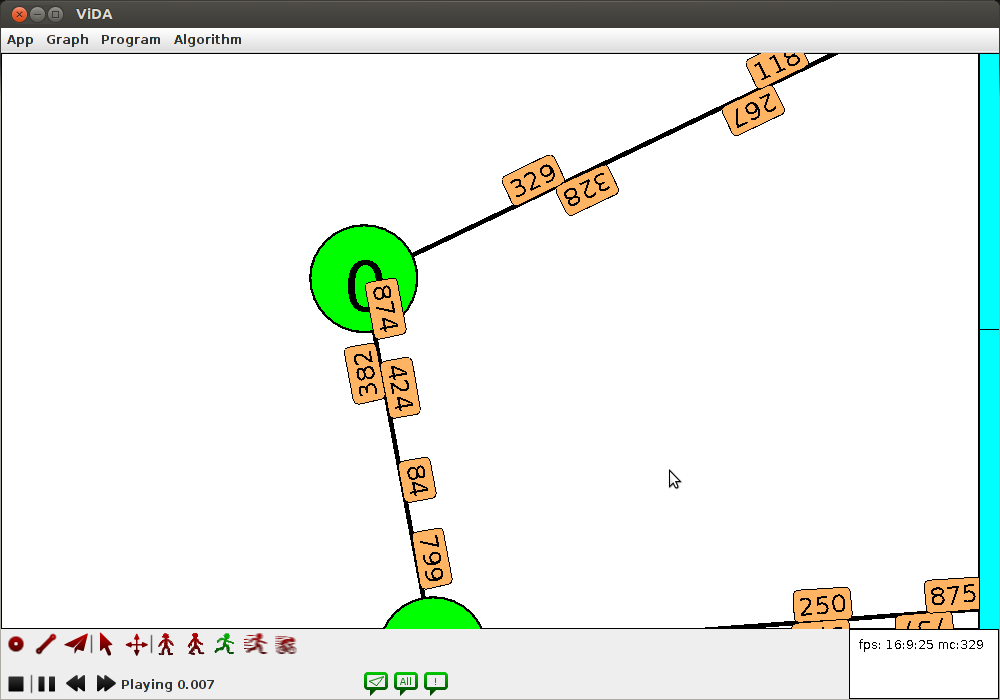
\includegraphics[width=\columnwidth]{spravy}

\mysection{Navizualizované algoritmy}

\begin{itemize}

    \item broadcast -- \textit{ako povedať novú klebetu všetkým v sieti?}
    \item traverzovanie -- \textit{ako len s pomocou jednej správy prehľadať celý graf?}
    \item voľba šéfa na úplnom grafe -- \textit{ako sa spomedzi niekoľkých identických programov
    dá zvoliť jeden šéf? a čo ak pri tom chceme poslať čo najmenej správ?}

\end{itemize}
    
\mysection{A}

%TODO aplikacia pred spustenim programu

\mysection{B}

%TODO zobrazovanie informacii za behu

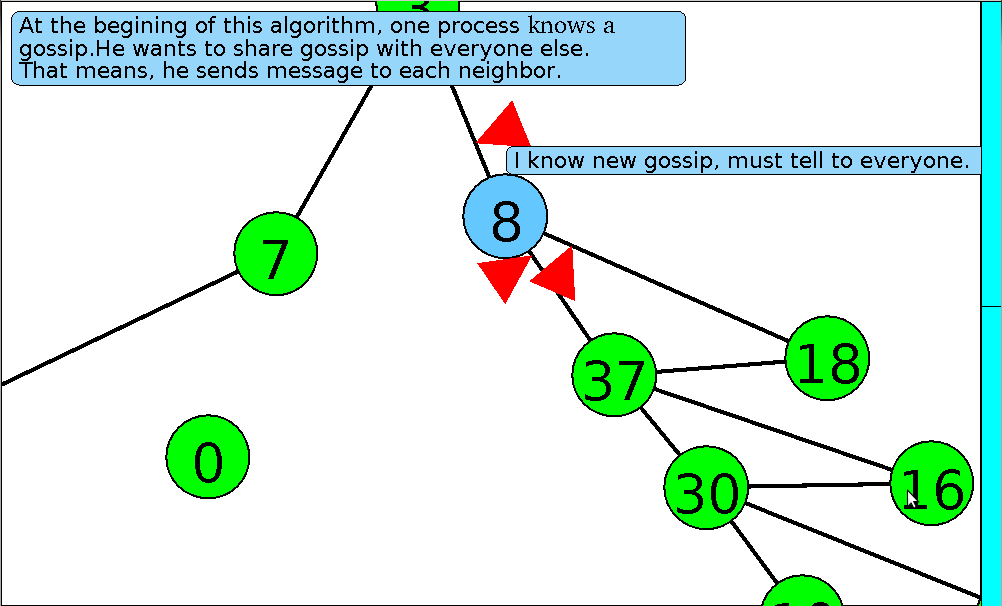
\includegraphics[width=\columnwidth]{bfs}

\mysection{C}

%TODO popis konkretnych algoritmov

\mysection{D}

%TODO plany do buducnosti
